

\section{Experiments}\label{sec:experiments}
%
In this section, we evaluate the performance of our methods with our competitors on real datsets.
% We will conduct experiments
We have implemented two variants of our methods (SPC and SPC*).
%for extracting statistics of queries, benchmarking the cost of a shortest path call,
%and selecting promising paths from a query log $\mathcal{QL}$ into the cache.
They share the same techniques in Section~\ref{sec:BenefitDriven},
and only differ in their cache structures:
(i) SPC uses a path array cache (Section~\ref{sec:cacheLookup}), and (ii) SPC* uses the compressed graph cache (Sections~\ref{sec:cacheSubgraph},\ref{sec:cacheCompress}).
%
Our competitors are LRU (a dynamic caching method) and HQF (a static caching method).
They have been introduced in Section~\ref{sec:competitors}.
All the above methods are written in C++.
We conduct our experiments on an Intel i7 3.4GHz PC running Debian.

%  (ii) SPC$^+$ uses a graph cache (Section~\ref{sec:cacheSubgraph}),
%SPC, our method, with the 3 cache representation schemes - List cache, Graph cache, Compressed Graph cache - described in section

We will evaluate the above methods for a cache located at the proxy, and for a cache located at the server.
For the proxy scenario, the performance measure is the hit ratio.
For the server scenario, the performance measures are: (i) the total running time of the server,
and (ii) the total number of road network nodes visited.


%in both the proxy
%well both when considering the Proxy and Server scenario

%To compare how well we have done, we have implemented two baseline competitors, LRU and HQF. LRU is a dynamic caching method which evicts the Least recently used cache item if there is no space in the cache for new entries. HQF adds to the cache, the \spaths from the most frequent start-/end-points in the training data.





%Aalborg: total nodes in SPs from training set: 352032 in 1643 paths

%Beijing: total nodes in SPs from training set: 316400 in 6479 paths



%This is the most common usage of static caching in the web caching literature \cite{BaezaYates07}.


% In this section, we present the results of performance
% experiments, demonstrating the efficiency and realworld applicability of the proposed algorithms. We


\subsection{Experimental Setting}
%
We are unable to obtain real query log from online shortest path services (e.g., Google Map), due to their privacy policies.
Thus, we can only simulate a query log from a trajectory dataset.
For each trajectory, we extract its start location and its end location as the
source $v_s$ and destination $v_t$ of a shortest path query respectively.

We have used two real datasets and their details can be found in Table~\ref{tab:datasetsize}.
Each dataset consists of (i) a collection of trajectories (which can be used to simulate a query log), and 
(ii) a corresponding road network for the trajectories.

%Which historical query datasets do we have, and what is their size and origin.

%- Aalborg: Query workload from and around the Danish city of Aalborg

%- Beijing: Query workload from Beijing



Following the experimental methodology of static caching~\cite{Ozcan2011},
we divide the query log into two equal sets.
The {\em historical query log} set is used for defining query frequencies and
for filling the cache content.
The {\em query workload set} set can only used for testing the performance of our method.


%We do not give a default size for the query-datasets Maps, as we will execute all of our tests, described in section \ref{subsec:expProxy} and \ref{subsec:expServer}, for each dataset.


\begin{table}
\center
\begin{tabular}{|c|r|r|r|}\hline
Dataset & $\#$ Trajectories / Queries & $\#$ Nodes & $\#$ Edges \\\hline
Aalborg & 4.401  & 129.680 & 137.470 \\\hline
Beijing & 12.928 & 76.226 & 85.882 \\\hline
\end{tabular}
\caption{Description of real datasets}
\label{tab:datasetsize}
\end{table}
%% Aalborg = Aalborg
%% Beijing = Beijing


%GPS trajectories

%according to XXX l

%The size of training and test query datasets are given already. The size of each dataset, as well as the map they are captured on, is given in table \ref{tab:datasetsize}.



%% Aalborg = Aalborg
%% Beijing = Beijing


%We do not give a default size for the query-datasets Maps, as we will execute all of our tests, described in section \ref{subsec:expProxy} and \ref{subsec:expServer}, for each dataset.




All caching methods, SPC, SPC*, HQF, and LRU, share a number of common settings which, unless stated otherwise, will be set to their default values:
The number of levels in the kD-tree is 14 (i.e. 16,384 regions). We will use the list cache representation as the default cache representation, where each vertex use one byte. The default cache size is set to 625 kB.


The default cache size, as well as the maximum cache size in later experiments (Fig.~\ref{fig:cSizeVsHitRatio}, \ref{fig:cacheSizeVsHitRuntime}, \ref{fig:cacheSizeVsNodesvisited}), is choosen baring in mind the size of the Aalborg and Beijing query logs. 
Had we had access to large datasets of real query logs, from online shortest path serveice providers, we would use a large cache size like 1 GB.

% 
% 
% The size of our datasets is the limiting factor
% 



\label{fig:cacheSizeVsHitRuntime}

\label{fig:cacheSizeVsNodesvisited}


% - Which parameters are common for all tests
% - What are the ranges/values each parameter can take.
% - Which parameters are set to a default value unless otherwise stated (and what are the default values)
% - Which methods, and in which configuration, do we consider.



\subsection{Caching in the Proxy Scenario}\label{subsec:expProxy}
%
In the proxy scenario, the shortest path call API would issue a shortest path query to the server,
rather than performing computation by itself (see Section~\ref{sec:benchmark}).
Since the total cost is dominated by the communication round-trip time with server,
we use the cache hit ratio as the performance measure in this scenario.

For both datasets we vary the cache size and kD-tree levels to show the impact on the cache hit ratio. We have implemented a number of optimizations to the cache storage (See sec. \ref{sec:CacheStruct}) and show their impact on the cache hit ratio.


\stitle{Effect of the cache size}
%
In Figure~\ref{fig:cSizeVsHitRatio}, we measure the hit ratio of the methods
while varying the cache size from 1 kB to 5 MB.


\begin{figure}[htb]
\center
  \begin{tabular}{@{}c@{ }c@{}}
     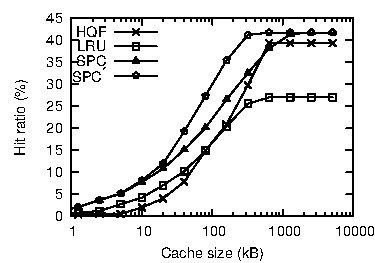
\includegraphics[width=0.5\columnwidth]{figures/cachesize_hitratio_aal.pdf}
     &
     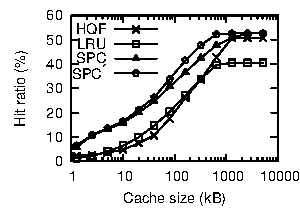
\includegraphics[width=0.5\columnwidth]{figures/cachesize_hitratio_bei.pdf}
      \\
     (a) Aalborg & (b)  Beijing
     \end{tabular}
\caption{Hit ratio vs. cache size }
\label{fig:cSizeVsHitRatio}
\end{figure}

% \begin{itemize}
% \item We can see SPC* performs much better than competitors
% \item LRU perform well on small cache sizes, but the cache hit ratio quickly level out and stop growing, thus LRU is not scalable.
% \item HQF performance is very consistent, with the hit ratio varying only slightly. The hit ratio does however stay at just over 1\% for Aalborg experiments and around 0.2\% for Beijing experiments. It is not usable
% \item We observe that SPC initially does not grow as fast as LRU, but the growth continues as we increase cache size, unlike for LRU.
% \item SPC* grows faster than LRU and gets better cache hit ratio at all cache sizes than LRU and SPC, except for the smallest cache size.
% \item The test on the Aalborg vs. Beijing sets show that SPC performs much better on the Aalborg set, where as LRU performs about 50\% worse. This can be explained by the fact that both methods rely on users behaving consistently over time, but where SPC relies on global consistency in user behavior, LRU need local consistency too. This makes SPC/SPC* more robust and we can expect them to always outperform LRU.
% \end{itemize}
{\color{red}
We can see that LRU consistently perform worse than SPC and SPC$^*$ for all cache sizes. The cache hit ratio stabilizes at about 26 and 40\% for Aalborg and Beijing respectively. Since LRU levels out at a much lower cache hit ratio than all of it's competitors it is not a suitable choice for \spath cacheing.


The performance of HQF is quite low at smaller cache sizes, 

The performance of HQF is very consistent, with the hit ratio varying only slightly. The hit ratio stays at just over 1\% for Aalborg experiments and around 0.2\% for Beijing experiments. The low hit ratio makes it not scalable and unusable for \spath caching.
}

SPC does not grow as fast as LRU for smaller cache sizes, but while the growth of LRU quickly stabilizes then SPC continues to grow and outperforms both LRU and HQF.
SPC* outperforms both LRU and SPC by a large margin, only shortly having a lower cache hit ratio at smaller cache sizes. The test on Aalborg vs. Beijing  show that SPC performs much better on the Aalborg set, where as LRU performs about 50\% worse. This can be explained by the fact that both methods rely on users behaving consistently over time, but where SPC relies on global consistency in user behavior, LRU need local consistency too. This makes SPC/SPC* more robust and we expect them to always outperform LRU.



\stitle{Effect of the kD-tree level}
%
In Figure~\ref{fig:levelVsHitRatio}, we vary the kD-tree level from 8 to 18 levels and show that using a kD-tree of about 14 levels can significantly increase the cache hit ratio of both the Aalborg and Beijing dataset. SPC* performs better than SPC.


\begin{figure}[htb]
\center
  \begin{tabular}{@{}c@{ }c@{}}
     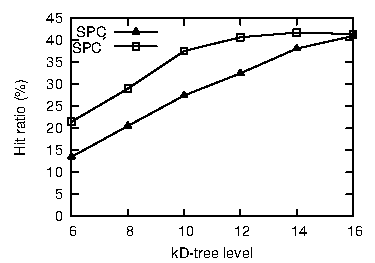
\includegraphics[width=0.5\columnwidth]{figures/split_hitratio_aal.pdf}
     &
     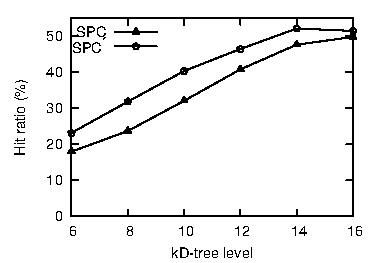
\includegraphics[width=0.5\columnwidth]{figures/split_hitratio_bei.pdf}
      \\
     (a) Aalborg & (b)  Beijing
     \end{tabular}
\caption{Hit ratio vs. Levels}
\label{fig:levelVsHitRatio}
\end{figure}

On both dataset SPC* outperforms SPC by a large margin. On the city X dataset SPC* achieves more than a 50\% increase in hit ratio, and when compared to SPC, it achieves a relative performance gain of 500-900\% at low levels up to the peak performance at level 14.
On the Y dataset SPC* gets a lower hit ratio, but it still achieves more than 50\% cache hit ratio. The results are still very impressive, with SPC* performing 200-400\% better than SPC at all levels.

% \noindent
% \begin{tabular}{|l |p{0.58\columnwidth} |l |}
% \hline
% \textbf{Parameter} & \textbf{Meaning / used for} & \textbf{Standard value} \\\hline
% Mapfile & The map which the test is performed on & \\\hline
% NumQueries & Number of \spath queries in test & \\\hline
% QuerySet & which dataset is used to provide queries & \\\hline
% TrainSet & For generating region statistics, which dataset is used & \\\hline
% CacheSize & Size of cache in bits & \\\hline
% cacheType & Type of cache representation (list/graph) & \\\hline
% kD-tree & Hight of the kD-tree & \\\hline
% avgLenght & Average length of a shortest path & \\\hline
% \end{tabular}

% Write experiments to examine performance of goal 1 \& 2
% Test ideas (several ideas may be combined, like item 1 can be done on all datasets from item 2):\\
% \begin{itemize}
% \item increase kd-tree hight from 0-18
% \item different maps [Oldenburg, Aalborg, Beijing]
% \item compare cache type performance
% \item compare with baseline methods. [LRU dynamic, Dynamic(maxLevel)]
% \item vary the cache size [10.000-2560000]
% \item vary number of queries. [only for synthetic data]
% \end{itemize}

\subsection{Caching in the Server Scenario}\label{subsec:expServer}
%
In the server scenario, the shortest path API has to invoke a shortest path algorithm.
Thus, the running time is the most important performance measure. We also measure the number of nodes visited in a shortest path algorithm, which serves an indicator of the running time.
%On a server our aim is slightly different than on the Proxy, as we also have to consider that there may be some paths that are so small that it may be cheaper to simply re-calculate the result, instead of caching it.
%For the server scenario we will test the cache hit ratio, running time, and Nodes visited.
%For all three experiments
%We will vary kD-tree levels and cache size in the following experiments.
As a case study, we use the Dijkstra's algorithm as the shortest path algorithm.

In the following experiments, the running time (and nodes visited) refer to the total running time (and nodes visited) for processing the entire query workload. The running time is measured in the unit of seconds.





\stitle{Estimation of shortest path running cost}
%
First, we test the estimation error of our cost estimation technique proposed in Section~\ref{sec:benchmark}.
We measure the error percentage in terms of the relative error between the actual cost and the estimated cost.
Table~\ref{tbl:estcost} shows the estimation error of our technique
as a function of: (a) the number of landmark $|U|$, and (b) the size of the samples $S$.
The default values are: $|U|=20$ and $S=100$.
The majority of errors are below 30\% and thus our estimation technique is reasonably accurate.


%% Aalborg: average cost = 136347/2 = 68173
%%  Beijing: average cost = 79603/2 = 39801
%  average because random node chosen



\begin{table}
\center
\begin{tabular}{cc}
    \begin{tabular}{|c|c|c|}
    \hline
    $|U|$ & Aalborg & Beijing \\ \hline \hline
     5 & 35.5 & 33.3 \\ \hline
     10 & 25.4 & 28.2 \\ \hline
     20 & 22.2 & 23.9 \\ \hline
     40 & 19.4 & 23.0  \\ \hline
     80 & 19.9 & 21.9 \\ \hline
    \end{tabular}
    &
    \begin{tabular}{|c|c|c|}
    \hline
    $S$ & Aalborg & Beijing \\ \hline \hline
     25 & 23.4 & 28.8 \\ \hline
     50 & 20.7 & 28.4 \\ \hline
     100 & 22.2 & 23.9 \\ \hline
     200 & 20.4 & 22.7 \\ \hline
     400 & 21.1 & 21.3 \\ \hline
    \end{tabular}
    \\
    (a) varying number of landmark $|U|$ & (b) varying sample size $S$
\end{tabular}
    \caption{Average error percentage of cost estimation}
    \label{tbl:estcost}
\end{table}








%
\stitle{Effect of the kD-tree level}
%
In Figure~\ref{fig:levelVsHitRatio}, we again vary the kD-tree level from 8 to 18 levels. All three experiments shows a consistent advantage of using SPC* over SPC. SPC* still has an even higher advantage than in the proxy scenario, performing around 950\% better than SPC at its best. SPC, however, has a very low hit ratio in the server scenario, on both the city X and Y datasets. In figure \ref{fig:levelVsruntime}a and b we can see that SPC* is very fast at answering the query workload. SPC has a quite stable time in both figure\ref{fig:levelVsruntime}a and b, while the time for SPC* to answer the query workload actually decreases with more regions. In figure \ref{fig:levelVsNodesvisited} we can see that SPC* visits far fewer nodes than SPC, during shortest path calculations. This is expected since SPC* can answer many more queries from its cache.




\begin{figure}[htb]
\center
  \begin{tabular}{@{}c@{ }c@{}}
     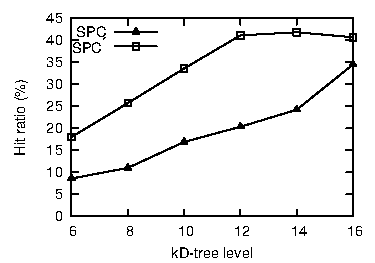
\includegraphics[width=0.5\columnwidth]{figures/split_hitratio_aal_server.pdf}
     &
     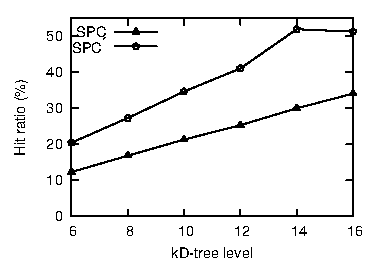
\includegraphics[width=0.5\columnwidth]{figures/split_hitratio_bei_server.pdf}
      \\
     (a) Aalborg & (b)  Beijing
     \end{tabular}
\caption{Hit ratio vs. Levels}
\label{fig:levelVsHitRatio}
\end{figure}

\begin{figure}[htb]
\center
  \begin{tabular}{@{}c@{ }c@{}}
     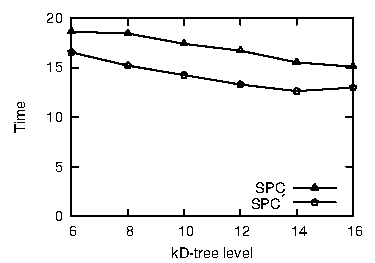
\includegraphics[width=0.5\columnwidth]{figures/split_runtime_aal_server.pdf}
     &
     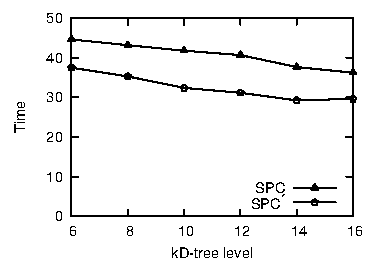
\includegraphics[width=0.5\columnwidth]{figures/split_runtime_bei_server.pdf}
      \\
     (a) Aalborg & (b)  Beijing
     \end{tabular}
\caption{Runtime vs. Levels}
\label{fig:levelVsruntime}
\end{figure}

\begin{figure}[htb]
\center
  \begin{tabular}{@{}c@{ }c@{}}
     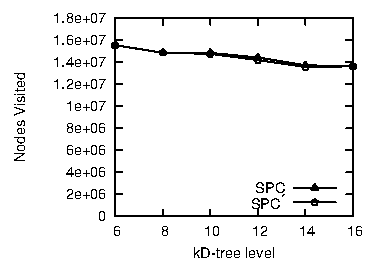
\includegraphics[width=0.5\columnwidth]{figures/split_nodes_aal_server.pdf}
     &
     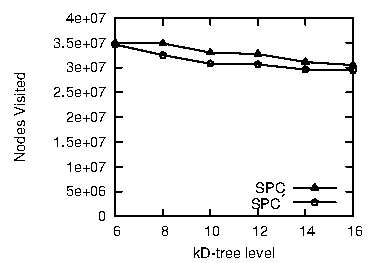
\includegraphics[width=0.5\columnwidth]{figures/split_nodes_bei_server.pdf}
      \\
     (a) Aalborg & (b)  Beijing
     \end{tabular}
\caption{Nodes Visited vs. Levels}
\label{fig:levelVsNodesvisited}
\end{figure}






\stitle{Effect of the cache size}
%
In the following experiments, we vary the cache size and observe the effect on the running time and nodes visited during shortest path calculations.






\begin{figure}[htb]
\center
  \begin{tabular}{@{}c@{ }c@{}}
     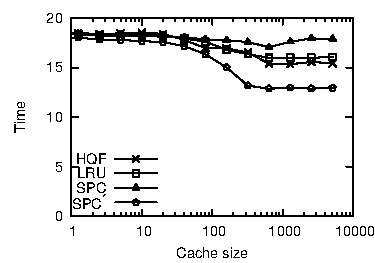
\includegraphics[width=0.5\columnwidth]{figures/cachesize_runtime_aal.pdf}
     &
     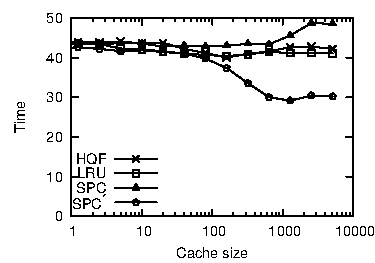
\includegraphics[width=0.5\columnwidth]{figures/cachesize_runtime_bei.pdf}
      \\
     (a) Aalborg & (b)  Beijing
     \end{tabular}
\caption{Runtime vs. Cache Size}
\label{fig:cacheSizeVsHitRuntime}
\end{figure}

In Figure \ref{fig:cacheSizeVsHitRuntime} and \ref{fig:cacheSizeVsNodesvisited}, for both the city X and Y dataset,  we can see that the graph looks similar to Figure \ref{fig:cSizeVsHitRatio}, but in the upside-down manner. This is to be expected, since a higher cache hit ratio gives fewer \spath calculations, and a lower runnig time when answering queries.

\begin{figure}[htb]
\center
  \begin{tabular}{@{}c@{ }c@{}}
     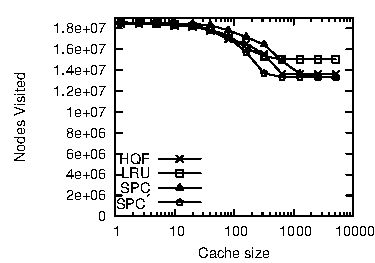
\includegraphics[width=0.5\columnwidth]{figures/cachesize_nodes_aal.pdf}
     &
     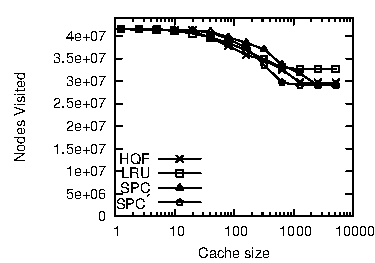
\includegraphics[width=0.5\columnwidth]{figures/cachesize_nodes_bei.pdf}
      \\
     (a) Aalborg & (b)  Beijing
     \end{tabular}
\caption{Nodes Visited vs. Cache Size}
\label{fig:cacheSizeVsNodesvisited}
\end{figure}
